\section{Geometry description file}
\label{sec:geom}
\noindent
The geometry description file provides
	\begin{itemize}
		\item the number of the meshed surfaces separating the different domains,
		\item  the names of the files corresponding to these surfaces,
		\item the number of domains of homogeneous conductivity,
		\item the positions of the domains with respect to the surfaces (inside or outside)
	\end{itemize}
The geometry description file should have as extension: *.geom

\centerline{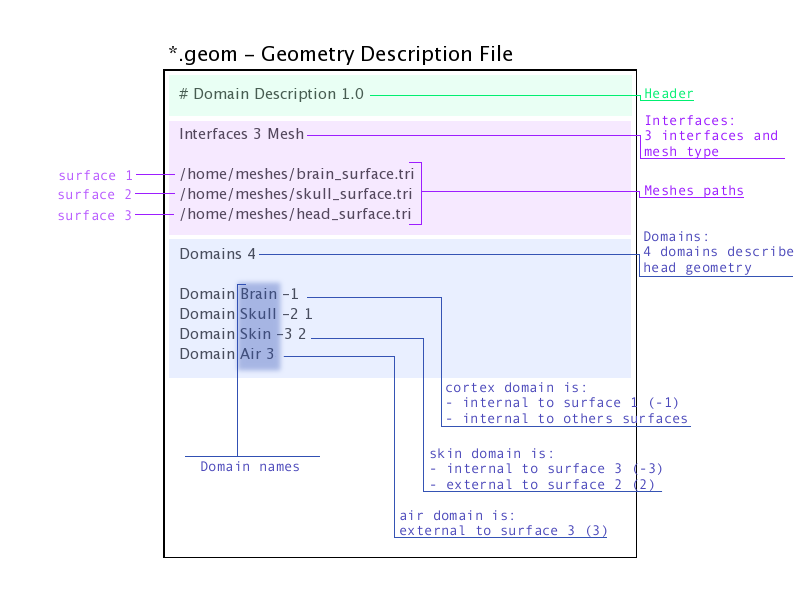
\includegraphics[height=9cm]{geom.png}}

\begin{note}
    	The domains are to be described in the following way (first the external surface and then the internal surface)~:

    \begin{tabular}{ll}
        Domain Brain -1              & \\
        Domain Skull \textbf{1 -2}	 &	\emph{and not Domain Skull -2 1} \\
        Domain Skin \textbf{2 -3}	 &	\emph{and not Domain Skin -3 2}  \\
        Domain Air 3                 &  \\
    \end{tabular}
\end{note}

\medskip

\begin{note}
    ``Meshes paths'' can be
    \begin{itemize}
        \item global (as on drawing)
        \item relative to where the command line is executed
    \end{itemize}
    For the meshes, the following formats are allowed~:
    \begin{itemize}
        \item *.tri~: TRI format corresponding to early BrainVisa. Also handled by Anatomist.
        \item *.mesh~: MESH format corresponding to BrainVisa versions 3.0.2 and later. Also handled by Anatomist.
        \item *.vtk~: VTK mesh format.
    \end{itemize}
\end{note}

%###################################################
\section{Conductivity description file}
\label{sec:cond}

\noindent
The conductivity description file defines the conductivity values corresponding to each domain listed in the Geometry Description File (section~\ref{sec:geom}).
\\
The file extension should be: *.cond .\\
\warning{  the domain names should match the ones defined in the Geometry Description File (beware of differences in upper/lower case).}


\centerline{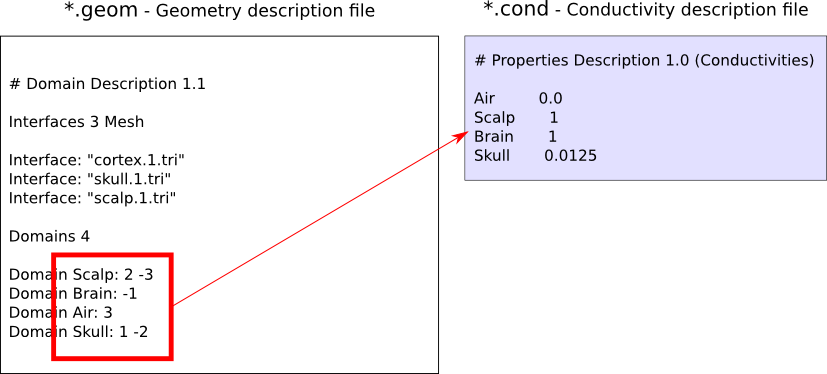
\includegraphics[height=9cm]{cond.png}}

%###################################################

\section{Source description}
Sources are defined by their geometry (position and orientation)  and their magnitude.
OpenMEEG handles two types of source models: isolated dipoles, or distributed dipoles: these two models differ in their geometry description.
%-----------------------------------
\subsection{Source position and orientation}
\label{sec:dipoles}
%---
\subsubsection{Isolated dipoles}
\noindent
Isolated dipoles are represented by a text file (extension *.dip or *.txt), in which each line defines a dipole position and orientation, encoded in 6 real values:

\begin{itemize}
    \item three values encoding the Cartesian coordinate for the position,
    \item three values encoding the orientation of the dipole (supposed unitary).
\end{itemize}

\medskip

\noindent
The following example shows a file describing 5 isolated dipoles:

\centerline{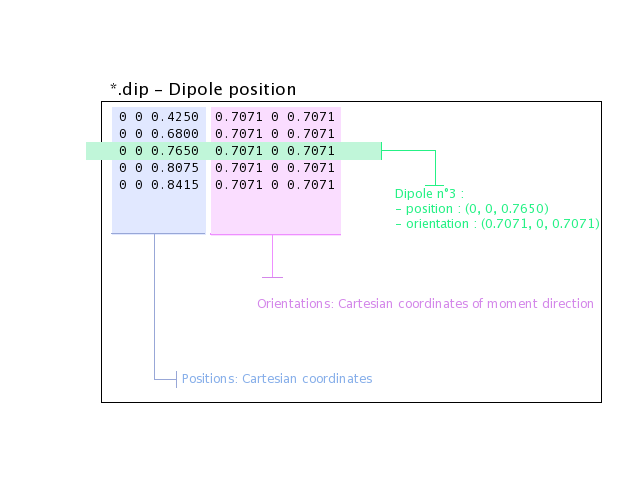
\includegraphics[height=9cm]{dipolePositions_en.png}}

\begin{note}
	The referential of the coordinates should be the same as for the meshes (the MR coordinates in general).
\end{note}
%---
\subsubsection{Distributed dipoles}
Distributed dipoles are supported on a mesh, whose format must be *.mesh, or *.tri, or *.vtk.
%-----------------------------------
\subsection{Source activation}
\label{sec:activ}

\noindent

Source activation files are text files, in which each line corresponds to a source, and each column to a time sample.
\begin{itemize}
    \item for isolated dipoles, the nth line corresponds to the amplitude of the nth dipole (with its fixed orientation)
    \item for distributed dipoles, the nth line correspond to the amplitude of the nth vertex in the source mesh.
\end{itemize}

\medskip

\noindent
Example for isolated dipoles:

\centerline{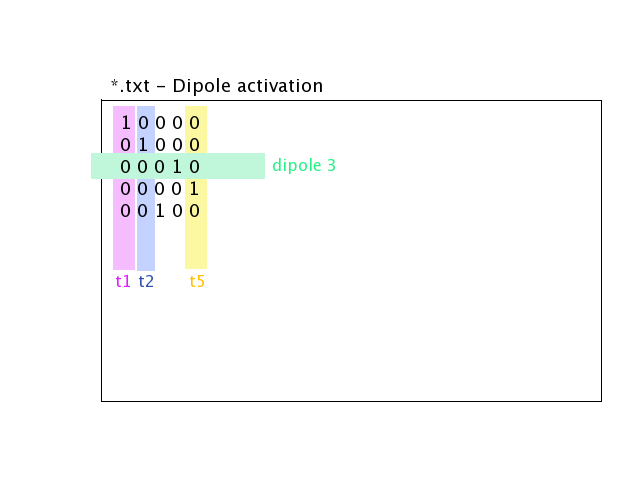
\includegraphics[height=9cm]{dipActiv.png}}

%###################################################

\section{Sensor definition}
\label{sec:sensors}

\noindent
The sensor definition is provided in a text file, in which each line provides the position of the sensor, and additional information such as its orientation or its name.
More precisely, there are 5 options for defining sensors:
\begin{enumerate}
\item  1 line per sensor and 3 columns (typically for EEG sensors or MEG sensors without orientation) :
	\begin{itemize}
		\item  the 1st, 2nd and 3rd columns are respectively position coordinates x, y, z of sensor
	\end{itemize}
\item  1 line per sensor and 4 columns (typically for EEG sensors or MEG sensors without orientation) :
	\begin{itemize}
		\item   the 1st column is sensors names
		\item the 2nd, 3rd and 4th are respectively position coordinates x, y, z of sensor
	\end{itemize}
\item 1 line per sensor and 6 columns (typically for MEG sensors) :
	\begin{itemize}
		\item  the 1st, 2nd and 3rd are respectively position coordinates x, y, z of sensor
		\item  the 4th, 5th and 6th are coordinates of vector orientation
	\end{itemize}
\item  1 line per sensor and 7 columns (typically for MEG sensors) :
	\begin{itemize}
		\item the 1st column is sensors names
		\item the 2nd, 3rd and 4th are respectively position coordinates x, y, z of sensor
		\item the 5th, 6th and 7th are coordinates of vector orientation
	\end{itemize}
\item 1 line per integration point for each sensor and 8 columns (typically for MEG realistic sensors with coils, or gradiometers) :
	\begin{itemize}
		\item  the 1st column is sensors names
		\item the 2nd, 3rd and 4th are respectively position coordinates x, y, z of sensor
		\item the 5th, 6th and 7th are coordinates of vector orientation
		\item  the 8th is the weight to apply for numerical integration (related to sensor name)
	\end{itemize}

\end{enumerate}

An example of MEG sensor description:

\centerline{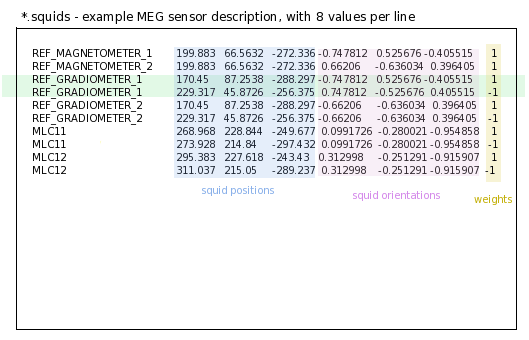
\includegraphics[height=9cm]{sensors-grad.png}}

%###################################################
